\documentclass[authordraft=true,dvipsnames]{acmart}

\usepackage{blindtext}
\usepackage{xpatch}
\usepackage{tikz}
\usepackage{subcaption}
\usepackage{pbox}
\usepackage{url}

\usetikzlibrary{matrix,backgrounds}
\pgfdeclarelayer{myback}
\pgfsetlayers{myback,background,main}

% By default the URLs are put in typewriter type in the body and the
% bibliography of the document when using the \url command.  If you are
% using many long URLs you may want to uncommennt the next line so they
% are typeset a little smaller.
\renewcommand{\UrlFont}{\small\tt}

%% Some hacks to remove all the ACM hardcoded text as I only want to use its style
\makeatletter
\xpatchcmd{\ps@firstpagestyle}{Manuscript submitted to ACM}{}{\typeout{First patch succeeded}}{\typeout{first patch failed}}
\xpatchcmd{\ps@standardpagestyle}{Manuscript submitted to ACM}{}{\typeout{Second patch succeeded}}{\typeout{Second patch failed}}    \@ACM@manuscriptfalse% Also in titlepage
\makeatother
\renewcommand\footnotetextcopyrightpermission[1]{} % removes footnote with conference info
\setcopyright{none}
\pagestyle{plain} % remove running headers
%% End of hack

%% Some shorthands
\newcommand{\pref}[1]{(\ref{#1})}
\newcommand{\bx}[0]{\mathbf{X}}
\newcommand{\bw}[0]{\mathbf{W}}
\newcommand{\by}[0]{\mathbf{Y}}
\newcommand{\bb}[0]{\mathbf{B}}

%% Drawing a cube in tikz
\newcommand{\tikzcube}[3]{% width, height, depth
\foreach \x in {0,...,#1}
{   \draw (\x ,0  ,#3 ) -- (\x ,#2 ,#3 );
    \draw (\x ,#2 ,#3 ) -- (\x ,#2 ,0  );
}
\foreach \x in {0,...,#2}
{   \draw (#1 ,\x ,#3 ) -- (#1 ,\x ,0  );
    \draw (0  ,\x ,#3 ) -- (#1 ,\x ,#3 );
}
\foreach \x in {0,...,#3}
{   \draw (#1 ,0  ,\x ) -- (#1 ,#2 ,\x );
    \draw (0  ,#2 ,\x ) -- (#1 ,#2 ,\x );
}
}

%% Highlight the elements in tikz matrix
\tikzset{mycolor/.style = {dotted,line width=1bp,color=#1}}%
\tikzset{myfillcolor/.style = {draw,fill=#1,opacity=0.3}}%

\NewDocumentCommand{\highlight}{O{blue!40} m m}{%
\draw[mycolor=#1] (#2.north west)rectangle (#3.south east);
}

\NewDocumentCommand{\fhighlight}{O{blue!40} m m}{%
\draw[myfillcolor=#1] (#2.north west)rectangle (#3.south east);
}

\title{Convolutional Layer and Its Matrix Implementation}
\author{Yinghai Lu}

\begin{document} 
\begin{abstract}
There are quite some tutorials~\cite{cs231n,andrew14,jefkin16} and textbooks~\cite{goodfellow16} explaining the mathematics of convolutional neural networks. However, in order to implement the CNN efficiently, we usually cast it into matrix operations. Few articles discuss this transformation process. \cite{cs231n} does a good job at the forward propagation pass but the backward propagation part is missing. In addition, many of them discuss simplified model with zero padding and $1$-stride. When I was reading the code of $CAFFE2$, I found myself constantly needing to figure out the all the parameters and all the indexing into the tensors. This notes tries to bridge the gap and provides a reference for matrix implementation of convolutional layer, consider various parameters and flavors. 
\end{abstract}
\maketitle

\section{Configuration}
The input to the convolutional layer is a 4D tensor $\bx \in \mathbb{R} ^{N \times C \times H_X \times W_X}$ (assuming NCHM format), which means a batch of $N$ images of size $H \times W$, where each image has $C$ channels. A set of $M$ filters of size $C \times H_K \times W_K$ will be applied to those input and generate the output $Y$. The filters are thus represented by a tensor $\bw \in \mathbb{R}^{M \times C \times H_K \times W_K}$. Optionally, we can have a bias vector $\mathbf{b} \in \mathbb{R}^{M}$, which offsets the result of the convolution. The output tensor $\by$ is of size $N \times M \times H_Y \times W_Y$, where the output image (activation map) dimension $H_Y \times W_Y$ is determined by configurations such as padding and stride and etc. 

For now, we assume zero-padding and stride of size $1$ for simplicity. We don't take group filters into account either. Later, we will see how to extend it. We also assume $N=1$ and omit the $n$ subscript. 

\section{Forward Propagation}
For a certain filter $m$, we drag it through the image to apply the convolution. Each time, we apply it onto a $H_K \times W_K$ tile of the image with $C$ channels and produce one element (pixel) in the output map:
\begin{equation} \label{forward}
\by_{m, i,j}=\sum_{c=0}^{C-1}{\sum_{p=0}^{H_K-1}{\sum_{q=0}^{W_K-1}{\bw_{m,c,p,q}\bx_{c, i+p,j+q}}}} + \mathbf{b}_m
\end{equation}

The above equation can be naturally converted to maxtrix multiplication. Let's first ignore the bias and focus on the convolution term. Given an input sample $\bx \in \mathbb{R}^{C \times H_X \times W_X}$, we are going to apply one filter $H_Y \times W_Y$ times by going from left to right and then from top to bottom. We introduce an operator $Im2Col()$ which takes  $\by$ as input and creates a 2D matrix $\bb \in \mathbb{R}^{(C \times H_K \times W_K) \times (H_Y \times W_Y)}$, where each column $B_{n,:,j}$ is made by reshaping the input area where the filter is going to be applied to into a $C \times H_K \times W_K$ column. As we are moving the filter, we are going to generate such a column $(H_Y \times W_Y$ times from left to right, top to bottom of the image. Here is an example of how we generate $\mathbf{B}$ from a $2 \times 3 \times 3$ input $\mathbf{X}$ with a $2 \times 2 \times 2$ filter kernel. 
\begin{figure}[h]
\begin{subfigure}[b]{0.3\textwidth}
\centering
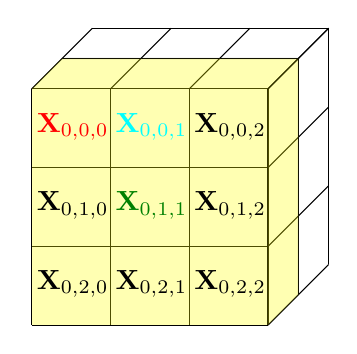
\begin{tikzpicture}[scale=1]
\tikzcube{3}{3}{2}
\draw[fill=Yellow,opacity=0.3] (0,0,2) -- (0,3,2) -- (3,3,2) -- (3,0,2);
\draw[fill=Yellow,opacity=0.3] (3,0,2) -- (3,0,1) -- (3,3,1) -- (3,3,2);
\draw[fill=Yellow,opacity=0.3] (0,3,2) -- (0,3,1) -- (3,3,1) -- (3,3,2);

\node at (-0.25, -0.25, 0) {$\bx_{0,2,0}$};
\node at (-0.25, 0.75, 0) {$\bx_{0,1,0}$};
\node at (-0.25, 1.75, 0) {\color{Red}{$\bx_{0,0,0}$}};
\node at (0.75, -0.25, 0) {$\bx_{0,2,1}$};
\node at (0.75, 0.75, 0) {\color{Green}{$\bx_{0,1,1}$}};
\node at (0.75, 1.75, 0) {\color{Cyan}{$\bx_{0,0,1}$}};
\node at (1.75, -0.25, 0) {$\bx_{0,2,2}$};
\node at (1.75, 0.75, 0) {$\bx_{0,1,2}$};
\node at (1.75, 1.75, 0) {$\bx_{0,0,2}$};
\end{tikzpicture}
\caption{Input $\bx$ of $2 \times 3 \times 3$}
\end{subfigure}
\hspace{20mm}
\begin{subfigure}[b]{0.3\textwidth}
\centering
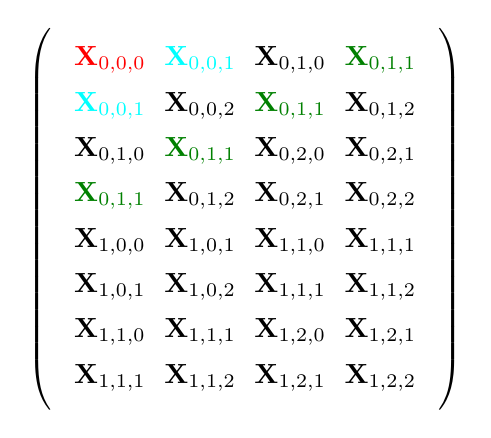
\begin{tikzpicture}[baseline=-\the\dimexpr\fontdimen22\textfont2\relax ]
\matrix(m)[matrix of math nodes,left delimiter=(,right delimiter=)]
{
\color{Red}{\bx_{0,0,0}} & \color{Cyan}{\bx_{0,0,1}} & \bx_{0,1,0} & \color{Green}{\bx_{0,1,1}}\\ 
\color{Cyan}{\bx_{0,0,1}} & \bx_{0,0,2} & \color{Green}{\bx_{0,1,1}} & \bx_{0,1,2}\\ 
\bx_{0,1,0} & \color{Green}{\bx_{0,1,1}} & \bx_{0,2,0} & \bx_{0,2,1}\\ 
\color{Green}{\bx_{0,1,1}} & \bx_{0,1,2} & \bx_{0,2,1} & \bx_{0,2,2}\\ 
\bx_{1,0,0} & \bx_{1,0,1} & \bx_{1,1,0} & \bx_{1,1,1}\\ 
\bx_{1,0,1} & \bx_{1,0,2} & \bx_{1,1,1} & \bx_{1,1,2}\\ 
\bx_{1,1,0} & \bx_{1,1,1} & \bx_{1,2,0} & \bx_{1,2,1}\\ 
\bx_{1,1,1} & \bx_{1,1,2} & \bx_{1,2,1} & \bx_{1,2,2}\\
};
\fhighlight[Yellow]{m-1-1}{m-4-4}
\end{tikzpicture}
\caption{$\bb = Im2Col(\bx)$ of $8 \times 4$ }
\end{subfigure}
\caption{An example of $Im2Col()$} \label{buffer} 
\end{figure}

With $\bb$, if we think the weight tensor as a 2D matrix of $M \times (C \times H_K \times W_K)$, where each row is just the filter map $m$ flattened, we can easily get the output of applying $\bw$ to $\bx$ as 
\begin{equation} \label{bm}
\by = \bw \bb
\end{equation}
where $\by \in \mathbb{R}^{M \times (H_Y \times W_Y)}$. 

Now we amend $\by$ to add bias term. What we want to do is to add $\mathbf{b}_i$ to each element in row $i$ of $\mathbf{Y}$. This can be done by generating a increament matrix and do element-wise add to  $\mathbf{Y}$:
\begin{equation} \label{bias}
 \mathbf{Y'} =  \by + \mathbf{b} \mathbf{u}^T
\end{equation}
where $\mathbf{u} \in \mathbb{R}^{(H_Y \times W_Y) \times 1}$ is a vector filled with $1$s. By doing an outer-product between $\mathbf{b}$ and $\mathbf{u}$, we strectch the incremental matrix we want and add it to $ \by$. Note that most numerical libraries offser GEMM routine which does operation in above equation in one call. 

Applying this to each of the input batch, we can get $\by$ for each $n \in \{0,\ldots,N-1\}$. 
 
\section{Backward Propagation}
For backward propagation, we are interested in generating the gradients for inputs ($d\bx$), for weights ($d\bw$) and for the bias terms ($d\mathbf{b}$). In addition to $\mathbf{X}$ and $\mathbf{W}$, we also know the output gradient back-propagated from next layer $d\by \in \mathbb{R}^{N \times M \times H_Y \times W_Y}$. We will focus on one sample of the input batch $N$ and hence omit the index $n$ in the following discussion.  

The gradient of weight $\bw_{m,c,p,q}$ with respect to the training error is about how much a perturbation in $\mathbf{W}_{m,c,p,q}$ is going to affect the output. It's worth noticing how much $\mathbf{W}_{m,c,p,q}$ is involved in the computation. Basically, for each filter $m$, if we have zero padding and stride of $1$, $\mathbf{W}_{m,c,p,q}$ will be involved in the computation of each pixel of the output activation map with respect to a specific filter and there are $H_Y \times W_Y$ of them. With that,  
applying the chain rule on the gradient and we get:
\begin{equation}
\frac{\partial E}{\partial \bw_{m,c,p,q}} = \sum_{i=0}^{H_Y-1}{\sum_{j=0}^{W_Y-1}{\frac{\partial E}{\partial \by_{m,i,j}}\frac{\partial \mathbf{Y}_{m,i,j}}{\partial  \mathbf{W}_{m,c,p,q}}}}
\end{equation}
Substituting $\by_{m,i,j}$ with \pref{forward}, we have
\begin{equation} \label{dw}
\frac{\partial E}{\partial \bw_{m,c,p,q}} = \sum_{i=0}^{H_Y-1}{\sum_{j=0}^{W_Y-1}{\frac{\partial E}{\partial \by_{m,i,j}}\bx_{c,i+p,j+q}}}
\end{equation}
 
For a given input of $d\by$ from a batch of $N$, we can treat it as a matrix $d\mathbf{Y}$ of size $M \times (H_Y \times W_Y)$. For each row $m$, each column represents an element $\mathbf{Y}_{m,i,j}$, flatterned into one row. Remember the buffer matrix $\bb=Im2Col(\bx)$ is a matrix of size $(C \times H_K \times W_K) \times (H_Y \times W_Y)$, we have 
\begin{equation}
d\bw = d\by \bb^T
\end{equation}
To see why, you can expand the matrix multiplication and verify that each element operation corresponds exactly to \pref{dw}.

Next, let's check the gradient of bias $\mathbf{b}_m$. Similar to $\bw_{m,c,p,q}$, $\mathbf{b}_m$ contributes to the computation of each of the pixels in an activation map of size  $H_Y \times W_Y$. Similarly, applying the chain rule and we have
\begin{equation}
\frac{\partial E}{\partial \mathbf{b}_m} =  \sum_{i=0}^{H_Y-1}{\sum_{j=0}^{W_Y-1}{\frac{\partial E}{\partial \by_{m,i,j}}\frac{\partial \mathbf{Y}_{m,i,j}}{\partial \mathbf{b}_m}}}
\end{equation}
From \pref{forward}, we know that $\frac{\partial \by_{m,i,j}}{\partial \mathbf{b}_m} = 1$. Therefore we have 
\begin{equation}
d\mathbf{b} = d\by \mathbf{u}
\end{equation}
where $\mathbf{u}$ is the vector with all ones, as we have already seen in \pref{bias}.

Finally, we still need to compute the gradient of input, $d\bx$. Using chain rule, the gradient of each input $\mathbf{X}_{c,i,j}$ is 
\begin{equation}
\frac{\partial E}{\partial \bx_{c,i,j}} = \sum_{p=0}^{H_K-1}{\sum_{q=0}^{W_K-1}{\sum_{m=0}^{M-1}{\frac{\partial E}{\partial \by_{m,i-p,j-q}}\frac{\partial \mathbf{Y}_{m,i-p,j-q}}{\partial \mathbf{X}_{c,i,j}}}}}
\end{equation}
Substituting \pref{forward} into the above euqation and we have
\begin{equation} \label{dx}
\frac{\partial E}{\partial \bx_{c,i,j}} = \sum_{p=0}^{H_K-1}{\sum_{q=0}^{W_K-1}{\sum_{m=0}^{M-1}{\frac{\partial E}{\partial \by_{m,i-p,j-q}} \bw_{m,c,p,q}}}}
\end{equation}
Note that the ranges of the three levels of summation show intuitively how a pixel $\bx_{c,i, j}$ contributes to the computation of output activation map $\by$. The outer two levels show that each pixel will be involved in computing (at most) $H_K \times W_K$ pixels in the activation map of one filtering, as is shown by the highlighted elements in Figure \pref{buffer}. And the innermost summation means that there are $M$ such filters. First, we can tackle the the innermost summation. 
Considering the following matrix $\bb^* \in \mathbb{R} ^ {C \times H_K \times W_K} \times (H_Y \times W_Y)$ 
\begin{equation} \label{rbb}
\bb^* = \bw^T d\by
\end{equation}
where each element in $B^*$ corresponds to a combination of $\sum_{m=0}^{M-1}{ \bw_{m,c,p,q}\by_{m,i,j} }$. Basically, $B^*$ gives the all the information we need to compute $d\bx_{c,i,j}$ and we can rewrite \pref{dx} to 
\begin{equation} \label{dx2}
\frac{\partial E}{\partial \bx_{c,i,j}} = \sum_{(a,b) \in A}{\bb^*_{a,b}}
\end{equation}

The problem is how to pick and choose the set $A$ so that the elements we choose satisfies \pref{dx}. Notice the structural similarity between $\bb^*$ and $\mathbf{B}$ in Figure \ref{buffer}. Both of them are of the same size and the elements are arranged in the same way. Since $\mathbf{B} = Im2Col(X)$, we can actually obtain $d\bx$ from $\mathbf{B}^*$ through a dual process of $Im2Col()$, which we call $Col2Im()$. What $Col2Im()$ does is the reverse process of $Im2Col()$, taking each column of the input matrix and patch it back to the output matrix of the same size of the input. Since patches overlap with each other, the values are added up, which corresponds to the summation in \pref{dx2}. The following Figure shows an example of how we reconstruct an element in $d\mathbf{X}$ from $\mathbf{B}^*$, where the input and kernl size are the same as the example in Figure \pref{buffer}. The colored boxes show how each column in $\mathbf{B}^*$ is stretched into a tile of pixels in $d\bx$. Note how the process is exactly the reverse of that in Figure \ref{buffer}.
\begin{figure}[h]
\begin{subfigure}[c]{0.5\textwidth}
\centering
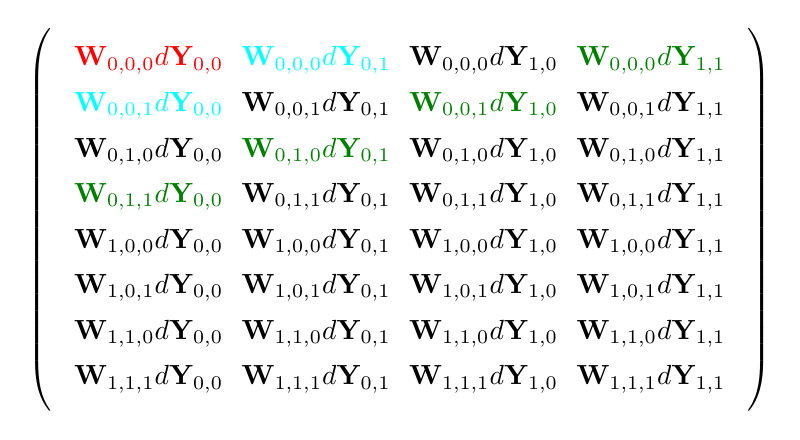
\begin{tikzpicture}[baseline=-\the\dimexpr\fontdimen22\textfont2\relax ]
\matrix(m)[matrix of math nodes,left delimiter=(,right delimiter=)]
{
\color{Red}{\bw_{0,0,0}d\by_{0,0}} & \color{Cyan}{\bw_{0,0,0} d\by_{0,1}} & \bw_{0,0,0}d\by_{1,0} & \color{Green}{\bw_{0,0,0}d\by_{1,1}}\\ 
\color{Cyan}{\bw_{0,0,1}d\by_{0,0}} & \bw_{0,0,1}d\by_{0,1} & \color{Green}{\bw_{0,0,1}d\by_{1,0}} & \bw_{0,0,1}d\by_{1,1}\\ 
\bw_{0,1,0}d\by_{0,0} & \color{Green}{\bw_{0,1,0}d\by_{0,1}} & \bw_{0,1,0}d\by_{1,0} & \bw_{0,1,0}d\by_{1,1}\\ 
\color{Green}{\bw_{0,1,1}d\by_{0,0}} & \bw_{0,1,1}d\by_{0,1} & \bw_{0,1,1}d\by_{1,0} & \bw_{0,1,1}d\by_{1,1}\\ 
\bw_{1,0,0}d\by_{0,0} & \bw_{1,0,0}d\by_{0,1} & \bw_{1,0,0}d\by_{1,0}& \bw_{1,0,0}d\by_{1,1}\\ 
\bw_{1,0,1}d\by_{0,0} & \bw_{1,0,1}d\by_{0,1} & \bw_{1,0,1}d\by_{1,0}& \bw_{1,0,1}d\by_{1,1}\\ 
\bw_{1,1,0}d\by_{0,0} & \bw_{1,1,0}d\by_{0,1} & \bw_{1,1,0}d\by_{1,0}& \bw_{1,1,0}d\by_{1,1}\\ 
\bw_{1,1,1}d\by_{0,0} & \bw_{1,1,1}d\by_{0,1} & \bw_{1,1,1}d\by_{1,0}& \bw_{1,1,1}d\by_{1,1}\\
};
\begin{pgfonlayer}{myback}
\highlight[Red]{m-1-1}{m-4-1}
\highlight[Blue]{m-1-2}{m-4-2}
\highlight[ForestGreen]{m-1-3}{m-4-3}
\highlight[Orange]{m-1-4}{m-4-4}
\end{pgfonlayer}
\end{tikzpicture}
\caption{$\bb^* = \bw^T d\by$ of $8 \times 4$ }
\end{subfigure} \\
\vspace{5mm}
\begin{subfigure}[c]{0.75\textwidth}
\centering
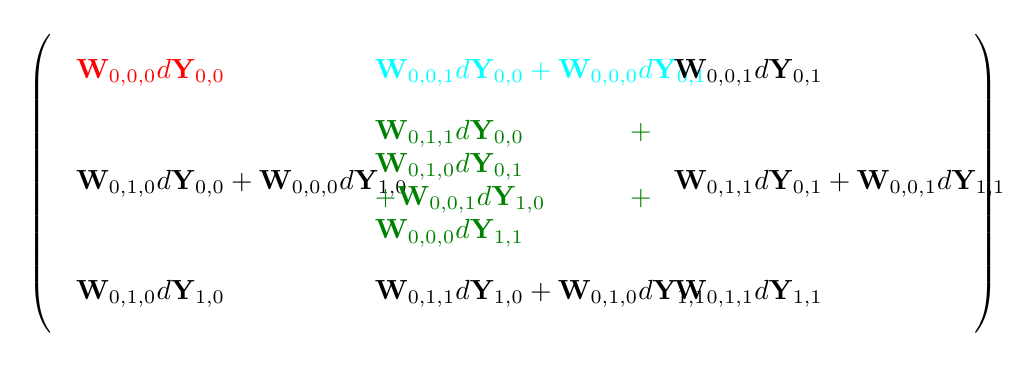
\begin{tikzpicture}[baseline=-\the\dimexpr\fontdimen22\textfont2\relax ]
\matrix(m)[matrix of math nodes,execute at begin cell = {\pbox[t]{\linewidth}}, left delimiter=(,right delimiter=), nodes={align=left, anchor=center, text width=100pt, minimum height=6ex, inner sep=4pt}]
{
\color{Red}{\bw_{0,0,0}d\by_{0,0}} & \color{Cyan}{\bw_{0,0,1}d\by_{0,0} + \bw_{0,0,0} d\by_{0,1}}  &  \bw_{0,0,1}d\by_{0,1} \\
\bw_{0,1,0}d\by_{0,0} +  \bw_{0,0,0}d\by_{1,0}  & { \color{Green}{$\bw_{0,1,1}d\by_{0,0} + \bw_{0,1,0}d\by_{0,1}$} \\ $+ \bw_{0,0,1}d\by_{1,0} + \bw_{0,0,0}d\by_{1,1}$} &  \bw_{0,1,1}d\by_{0,1} +  \bw_{0,0,1}d\by_{1,1} \\
 \bw_{0,1,0}d\by_{1,0} & \bw_{0,1,1}d\by_{1,0} +  \bw_{0,1,0}d\by_{1,1}  &   \bw_{0,1,1}d\by_{1,1} \\
};
\begin{pgfonlayer}{myback}
\highlight[Red]{m-1-1}{m-2-2}
\highlight[Blue]{m-1-2}{m-2-3}
\highlight[ForestGreen]{m-2-1}{m-3-2}
\highlight[Orange]{m-2-2}{m-3-3}
\end{pgfonlayer}
\end{tikzpicture}
\caption{First channel of $d\bx = Col2Im(\bb^*)$ of $2 \times 3 \times 3$}
\end{subfigure}
\caption{An example of $Col2Im()$ \label{dual}}
\end{figure}

\section{Different Flavors}
Normally, convulational layer will be configured to be more than just zero padding and stride $1$. Hence, we discuss how to take those parameters into consideration. 

\subsection{Padding, Stride and Dilation}
The beauty of $Im2Col()$ is that it abstracts away how we grab the pixels from the input to form the receptive field for convolution. Padding, stride and dilation all just change the way we grab the pixels and is taken care of by the $Im2Col()$ function. Padding tells $Im2Col()$ if the pixels are padded one, just put $0$ into $\bb$. Stride tells $Im2Col()$ how to move the convolution window around. And dilation tells $Im2Col()$ to strech the receiptive field and collect pixels that corresponds to non-zero weights. Since $Col2Im()$ is just a reverse process of $Im2Col()$, it will also take padding, stride and dilation into consideration. The core of the computation, i.e. the matrix multiplications, does not change.  

Another important influence of padding ($P$), stride ($S$) and dilation ($D$) is that they determine the size of output image, i.e. $H_Y$ and $W_Y$, which has been missing in the discussion. With some geometry intuition, we can see that
\begin{eqnarray}
H_Y &=& (H_X + P_T + P_B - (D_H * (H_K - 1) + 1)) / S_H + 1 \\
W_Y &=& (W_X + P_L + P_R - (D_W * (W_K - 1) + 1)) / S_W + 1 
\end{eqnarray}
where $P_{\{T,B,L,R\}}$ are paddings from top, bottom, left and right, and $D_{\{H,W\}}$ and $S_{\{H,W\}}$ are dilation and stride along height and width direction. 

\subsection{Group Filters}\footnote{Group filters currently don't work with dilated convolution in $CAFFE2$}
\cite{alexnet} introduces group filters to reduce the number of weight so that the computation can fit into the configeration of GPUs. In addition, it seems that group filters can actually improve the accuracy, and the resulting trained filters look more intuitive when plotted as 2D images. For group filters, we partition a set of $M$ filters groups of $G$, and there will be $M/G$ groups. Each filter in a group, intead of working on all the $C$ channels, works on $C/G$ channels. For all the filters that work on group $g \in \{0,\ldots,M/G-1\}$, we collect them together to form a matrix of size $(M/G) \times ((C/G) \times H_K \times W_K)$.
\begin{equation*}
\bw_g = [\mathbf{w}_{g \times M/G}^l, \mathbf{w}_{g\times M/G+1}^l, \ldots, \mathbf{w}_{(g+1) \times M/G-1}^{l}]^T
\end{equation*}
where $\mathbf{w}_g^l$ means a filter $g$-th group and works on the input channel $[l\times C/G, (l+1)\times C/G-1]$.

In addition, we need to tell the $Im2Col()$ function to grab pixels from $C/G$ instead of $G$ channels to form the buffer matrix $\bb_g$ and its resulting size will be $(C/G \times H_K \times W_K) \times (H_Y \times W_Y)$. Similar to~\pref{bm}, output regarding to this group of filters can be computed as 
\begin{equation} \label{bmg}
\by_g = \bw_g \bb_g
\end{equation}
Note that $\by_g \in \mathbb{R} ^ {(M/G) \times H_Y \times W_Y}$. Repeat this for $g \in \{0,\ldots,M/G-1\}$ and combine the results together and you will get $\mathbf{Y}$.

\section{Locally-Connected Layer}
In conventional convolutional layers, the weights of a filters are shared among computation of all the pixels of the output map. In other words, we use this same filter to scan the whole image to extract feature. It makes sense in the case of general images because the objects in interest can appear anywhere in the image. However, for some specific applications such as face recognition, this may not be a good idea, because the input of the face recognition is the frontal face photo where specific features such as eyes and mouth exist in specific region of the image. In this case, we do not want to share the weights of the filters at each location of convolution. We call convolutional layer without weight sharing locally-connected layer.

\subsection{Forward Propagation}
With out weight sharing, \pref{forward} becomes 
\begin{equation}
\by_{m, i,j}=\sum_{c=0}^{C-1}{\sum_{p=0}^{H_K-1}{\sum_{q=0}^{W_K-1}{\bw_{m,c,p,q,i,j}\bx_{c, i+p,j+q}}}} + \mathbf{b}_{m,i,j}
\end{equation} 
Notice the additional indices $i,j$ in the weights and biases. Since we have different set of weights for each of the $H_Y \times H_W$ convolutional locations. The input weight tensor is now of size $M  \times C \times H_K \times W_K \times H_Y \times W_Y$. Similarly, bias becomes a tenor of size $M \times H_Y \times W_Y$. However, the output $\by$ is still of the same dimension ($N \times M \times H_Y \times W_Y$). Again, we will assume $N=1$ and omit the first dimension in the following discussion.

First, we can still use $Im2Col()$ to take care of the padding, stride and dilation and prepare the buffer matrix $\bb  \in \mathbb{R}^{(C \times H_K \times W_K) \times (H_Y \times W_Y)}$. However, we cannot do direct matrix multiplication with parts of $\bw$ and $\mathbf{B}$ because it will create terms $\bw_{m,c,p,q,i,j}\bx_{c, i+p,j+q}$ where $i \neq j$. Instead, if we arrange $\bw$ into $\bw_m \in \mathbb{R} ^{(C \times H_K \times W_K) \times (H_Y \times W_Y)}$ for $m=0,\ldots,M-1$, we can use Hadamard product to compute the first term of the output, ignoring the bias for now:
\begin{equation} \label{ym2}
\by_m = \mathbf{u}^T (\bw_m \odot \bb)
\end{equation}
where $\odot$ denotes the Hadamard product (element-wise product) and $\mathbf{u}$ is the same all one vector of size $C \times H_K \times W_K$. The result $\by_m$ is a $H_Y \times W_Y$ vector. Repeating this for all $m$ and assemble the result, and we will get $\by$. Some remarks: 
\begin{enumerate}
\item When repeating~\pref{ym2} $M$ times, in terms of complexity, it is the same as matrix multiplication in~\pref{bm}. But we are making $2M$ calls ($M$ for Hadamont product and $M$ for AXPY) instead of $1$. This may introduce inefficiency compared to the weigth sharing convolutional layer. 
\item cuBLAS and Intel MKL provide support for Hadamond product (DHAD, vdMul) but OpenBLAS doesn't yet~\cite{openblas}. This is not a hard blocker though because it is fairly easy to add this considering OpenBLAS already has elementwise addition. 
\item The AXPY operation with $\mathbf{u}$ in~\pref{ym2} is an overkill. Effectively, we just need a reduction operation. BLAS provides ASUM operation for that. If there is support for that in CUDA, we can just use that. 
\item We can actually convert the Hadamard product to matrix multiplication by creating a huge block-diagnal matrix. BLAS has built-in support for diagnal matrix but I am not sure whether this will help us in terms of performance or not. 
\end{enumerate}

Next, we add the bias terms. Since $Y$ and $\mathbf{b}$ are of the size shape. Adding the bias is as simple as a matrix addition
\begin{equation}
\by' = \by + \mathbf{b}
\end{equation}

\subsection{Backward Propagation}
The input of gradient propagation is the same as normal convulational layer where we have $\bx$, $\bw$ and $d\by$, except for that $\bw$ is of size $M  \times C \times H_K \times W_K\times H_Y \times W_Y$ and $\mathbf{b}$ is of size $M \times H_Y \times W_Y$. For output, $d\bw$ will be the same size as $\bw$ and bias gradient $d\mathbf{b}$ will be the same size of $\mathbf{b}$. $d\bx$ will keep the same size as input $N \times C \times H_X \times H_Y$.

First, we compute the gradient of the weight $\bw_{m,c,p,q,i,j}$. Note that for a given filter $m$, each set of weight for each convolutional operation only contributes to one pixel in the output activation map, instead of $H_Y \times W_Y$ of them. Therefore, we have
\begin{equation}
\frac{\partial E}{\partial \bw_{m,c,p,q,i,j}} = \frac{\partial E}{\partial \by_{m,i,j}} \frac{\partial \by_{m,i,j}}{\partial  \bw_{m,c,p,q,i,j}} =  \frac{\partial E}{\partial \by_{m,i,j}} \bx_{c,i+p,j+q}
\end{equation}
Notice that compared to~\pref{dw}, it is a single multiplication instead of a convulation. Again, we will iterate through filter $m=0,\ldots,M-1$ and suppose we already have $\bb=Im2Col(\bx)$. Considering $d\by$ a $M \times (H_Y \times W_Y)$ matrix, and $\mathbf{B}$ and matrix of size $(C \times H_H \times W_K) \times (H_Y \times W_Y)$,  
\begin{equation*}
d\bw_{m,c,p,q,:,:} = \by_{m,:} \odot \bb_{k,:}
\end{equation*}
computes a vector of $H_Y \times W_Y$ weights, where we first iterate on each row of $\by$ for $m=0,\ldots,M-1$ and then on each row of $\bb$ for $k=0,\ldots,C\times H_K \times W_K$. There will be $M \times C \times H_K \times W_K$ Hadamard product of size $H_Y \times W_Y$. 

 
Similarly, the bias gradients can be propagated as 
\begin{equation}
\frac{\partial E}{\partial \mathbf{b}_{m,i,j}} = \frac{\partial E} {\partial \by_{m,i,j}} \frac{\partial \by_{m,i,j}} {\partial \mathbf{b}_{m,i,j}} = \frac{\partial E} {\partial \by_{m,i,j}} 
\end{equation}
So literally, $d\mathbf{b}=d\by$.

Finally, we compute the input gradient $d\bx$. A pixel in input $\bx_{c,i,j}$ still contributes to the computation of output activation map $\by$ in locally connected layer the same way as that in convolutional layer does. However, the weigths are a bit different. The formula to compute $d\bx_{c,i,j}$ is as follows
\begin{equation}
\frac{\partial E}{\partial \bx_{c,i,j}} = \sum_{p=0}^{H_K-1}{\sum_{q=0}^{W_K-1}{\sum_{m=0}^{M-1}{\frac{\partial E}{\partial \by_{m,i-p,j-q}}\frac{\partial \mathbf{Y}_{m,i-p,j-q}}{\partial \mathbf{X}_{c,i,j}}}}} = \sum_{p=0}^{H_K-1}{\sum_{q=0}^{W_K-1}{\sum_{m=0}^{M-1}{\frac{\partial E}{\partial \by_{m,i-p,j-q}} \bw_{m,c,p,q,i,j}}}} 
\end{equation}
The idea is the same as computing $d\bx$ in convulational layer. We want to compute a buffer matrix $\bb^*$ similar to~\pref{rbb} first and get $d\bx = Col2Im(\mathbf{B}^*)$, where each element in $\mathbf{B}^*$ corresponds to $\sum_{m=0}^{M-1}{\bw_{m,c,p,q,i,j}\by_{m,i,j}}$. Observe each element in $\bb^*$ in Figure~\ref{dual} presents multiplication between $\bw$ and $d\by$ along kernel pixel index as the row index increases and along output pixel index as the column index increases. The difference is that for each column, we have different weights. In order to do that, we first initialze $\mathbf{B}^*$ to be all zero.  
Next, we iterate on $m=0,\ldots,M-1$ and arrange $\bw$ into $M$ chunks of $\bw_m$ (same as in~\pref{ym2}). Then, we iterate on the rows of $\bw_m$:
\begin{equation*}
\bb^*_{k,:} = \bb^*_{k,:} + \bw_{m_{k,:}} \odot d\by_{m,:}
\end{equation*}
where $k=0,\ldots, C \times H_K \times W_K$. Repeating the process by $M$ times and we will obtain the final result of $\bb^*$. With that, we can obtain $d\bx$ by applying $Col2Im(\bb^*)$. 

\subsection{Efficient implementation with Batched GEMM}
From last section, we see that computing the forward and backward propagation usually involves $M$ alls to Hadamard product, which may require multiple kernels calls when implemented on GPU, which is suboptimal. Both Intel MKL and cuBLAS supports an operation called $BatchedGEMM$. $BatchedGEMM$ in a simpled form takes two tensor input $A \in \mathbb{R} ^{N \times P \times Q}$ and $B \in \mathbb{R}^{N \times Q \times R}$ and produce an output tensor $C \in \mathbb{R}^{N \times P \times R}$, where
\begin{equation*}
C_{n, :, :} = A_{n, :, :} B_{n, :, :}
\end{equation*}
It is one single kernel call to the GPU. 

To take advantage of that when computing the forward propagation, we now reshape $\bw$ to be of size $H_Y \times W_Y \times M \times C \times H_K \times W_K$. We partition it into $H_Y \times W_Y$ matrices $\bw_k$ of size $M \times (C \times H_K \times W_K)$ and iterate on $k$. Each iteration yields $M$ results of $\by$ on the same convolution location:
\begin{equation*}
\by'_{i,j,:} = \bw_k \bb_{:,k}
\end{equation*}
Basically, we can implement this with one call to $BatchedGEMM(\bw, \bb^T)$, where $\bw$ is considered a 3D tensor of size $(H_Y \times W_Y) \times M \times (C \times H_K \times W_K)$ and $\bb^T$ is considered of size $(H_Y \times W_Y) \times (C \times H_K \times W_K) \times 1$. Notice that $\by'$ is of size $H_Y \times W_Y \times M$, we might need to reshape it into $\by$.

For backward propagation of weight gradients, similarly, we will iterate over output pixels $H_Y \times W_Y$ and use that as our batch size to call $BatchedGEMM$. For each $k=0,\ldots,H_Y \times W_Y-1$, we take a column of $d\by$ and a column of $\bb$ and computes their outer product, which yields a matrix of $M \times (C \times H_K \times W_K)$ weight gradients $d\bw_{i,j,:,:,:,:}$. Implementation is basically one call to $BatchedGEMM(d\by^T, \bb)$, where $d\by^T$ is considered of size $(H_Y \times W_Y) \times M \times 1$.

Finally, for backward propagation of input gradients, we focus on how to compute $\bb^*$ with $BatchedGEMM$. Again, we use slices of input weight $\bw_k$, for $k=0,\ldots,H_Y \times W_Y -1$. In each iteration 
\begin{equation*}
\bb^*_{:,k} = \bw_k^T d\by_{:,k}
\end{equation*}
generates one column of $\bb^*$. The whole operation can be wrapped with one call to $BatchedGEMM(\bw_k^T, d\by^T)$. Similarly, resulting $\bb^*$ needs reshaping before applying $Col2Im$ to it. 

%\section{Tiled Convulational Layer}

\bibliographystyle{IEEEtran}
\bibliography{cnnref} 

\end{document}
